% MAIN-DOCUMENT

% Header beinhaltet Dokumentenklasse sowie includierte Packages
%KOMA-Script-Klasse: scrreprt
%deutsches Design, Schriftgröße 12, DIN A4
\documentclass[12pt,a4paper,oneside]{scrreprt}
%Seitenspiegel einstellen
\usepackage[a4paper]{geometry}
\geometry{a4paper,left=30mm,right=25mm,
bottom=20mm,top=15mm,bindingoffset=2mm,
includehead,includefoot}



%schalte Umlaute frei
\usepackage[ngerman]{babel}
%passende Codierung
\usepackage[utf8]{inputenc}
%Seitenspiegel einzustellen
\usepackage[a4paper]{geometry}
%Mathepaket
\usepackage{amsmath}
%Symbole
\usepackage{amssymb}
%griechische Symbole
\usepackage{upgreek}
%weitere Symbole
\usepackage{pxfonts}
% Phonetischen Alphabete für LaTeX
\usepackage{tipa}
%farbige Schriften
\usepackage{xcolor}
\usepackage{scrhack}
%Bilder fixieren
\usepackage{float}
%Grafiken einbinden
\usepackage{graphicx}
% Kopf- und Fußzeilen
\usepackage[automark,standardstyle,markusedcase]{scrpage2}
% deutsche Überschriften
\usepackage[ngerman]{translator}
% Kopfzeilenabstand festlegen
\setlength{\headheight}{10mm}
%Abb. statt Abbildung
\usepackage{caption3}
%klickbare Referenzen
\usepackage{hyperref}
%Quellcode Format
\usepackage{listings}
%draft Wasserzeichen
\usepackage{draftwatermark}
\SetWatermarkLightness{0.95}
\addto\captionsngerman{
\renewcommand{\figurename}{Abb.}
\renewcommand{\tablename}{Tab.}
}
%Glossar-Pakage
\usepackage[
nonumberlist, %keine Seitenzahlen anzeigen
acronym,      %ein Abkürzungsverzeichnis erstellen
toc]          %Einträge im Inhaltsverzeichnis      
{glossaries}
\usepackage{cite}
%Glossar einschalten
\makeglossaries



%Einstellungen Kopfzeile
\pagestyle{scrheadings} 
\setheadsepline{0.4pt}
\pagestyle{scrheadings}
\renewcommand*{\chapterpagestyle}{scrheadings}

%Zeilenabstand * 1.25 (default)
\renewcommand{\baselinestretch}{1.25}\normalsize


\begin{document}

% TODO: Glossar

%Titelseite

% Seitennummer aus
\thispagestyle{empty}


\begin{titlepage}

\vspace{3cm}

\begin{center}
    
\includegraphics[scale=0.8]{Titelseite/hl-logo.pdf}  
\end{center}

\vspace{2.5cm}

\begin{center}
\Large FAKULTÄT INFORMATIK
\end{center}

\vspace{1cm}
\begin{center}
    \Huge
    \textbf{Bachelorarbeit}\\
\end{center}

\vspace{1cm}

\begin{center}
    \Large
    \textsc{Programmieren in Rust und Vergleich mit C/C++}\\
\end{center}

\vspace{1.5cm}

\begin{center}
    \Large
    Thomas Keck
\end{center}

\vspace{4cm}
\begin{center}
    \large
    Betreuer: Prof. Dr. rer. nat. Dieter Nazareth
\end{center}

\end{titlepage}

\clearpage
\ifodd\count0\else
\thispagestyle{empty}
\hbox{}\newpage
\fi

%Erklärung
\thispagestyle{empty}
\vspace{15mm}
\begin{center}
\textbf{\underline{ERKLÄRUNG ZUR BACHELORARBEIT}}
\end{center}
\vspace{25mm}
\begin{center}
\large
Keck, Thomas
\end{center}
\vspace{25mm}

\begin{center}
\huge
Hochschule Landshut \\
Fakultät Informatik 
\end{center}
\vspace{10mm}

\begin{center}
\large
Hiermit erkläre ich, dass ich die Arbeit selbständig 
verfasst, noch nicht anderweitig für Prüfungszwecke 
vorgelegt, keine anderen als die angegebenen Quellen 
oder Hilfsmittel benützt, sowie wörtliche und sinngemäße 
Zitate als solche gekennzeichnet habe.  \\
\end{center}
\vspace{55mm}

\begin{center}
....................\hspace{40mm}....................................................\\

(Datum)\hspace{47mm}(Unterschrift des Studierenden)
\end{center}

\clearpage
\ifodd\count0\else
\thispagestyle{empty}
\hbox{}\newpage
\fi

% TODO: Abstract

% Liste Menüpunkte als Inhaltsverzeichnis
\tableofcontents
\setcounter{page}{1}

% Kapitel
\chapter{Einleitung}


\section{Was ist Rust?}

Rust ist eine quelloffene System-Programmiersprache, die sich auf Geschwindigkeit, Speichersicherheit und Parallelität konzentriert. Entwickler nutzen Rust für ein breites Spektrum an Anwendungsgebieten: Spiel-Engines\footnote{http://arewegameyet.com}, Betriebssysteme\footnote{z. B. Redox OS}, Dateisysteme und Browserkomponenten. \cite{Rust}

Eine aktive Gemeinschaft von Programmierern verwaltet die Codebasis und fügt fortlaufend neue Verbesserungen hinzu. Mozilla sponsert das Open-Source-Projekt.

Rust wurde von Grund auf neu aufgebaut und enthält Elemente aus bewährten und modernen Programmiersprachen. Es verbindet die ausdrucksstarke und intuitive Syntax von High-Level-Sprachen mit der Kontrolle und Leistung einer Low-Level-Sprache. Es verhindert Segmentierungsfehler und gewährleistet Threadsicherheit. Dadurch können Entwickler Code schreiben, der ehrgeizig, schnell und korrekt ist.

Rust macht die Systemprogrammierung durch die Kombination von Leistung und Ergonomie zugänglicher. Es bietet starke Features wie Zero-Cost-Abstraktionen, sichere Speicherverwaltung durch einen strengen Compiler und Typsystem sowie risikolose Nebenläufigkeit.

Große und kleine Unternehmen setzen Rust bereits ein, darunter:
\begin{itemize}
    \item Mozilla: Wichtige Komponenten von Mozilla Firefox Quantum.
    \item Dropbox: Mehrere Komponenten wurden in Rust als Teil eines größeren Projekts geschrieben, um eine höhere Effizienz des Rechenzentrums zu erreichen.
    \item Yelp: Ein Framework für Echtzeit A/B-Tests, welches auf allen Yelp-Websites und -Anwendungen verwendet wird.
\end{itemize}

\chapter{Rust toolchain}

Die Rust toolchain ist eine Sammlung von Werkzeugen, die dabei helfen, den Compiler aktuell zu halten und Projekte zu verwalten.


\section{rustup}

Das Rustup-Tool ist die empfohlene Installationsmethode für Rust. Das Tool ermöglicht zusätzlich die Verwaltung von verschiedenen Versionen, Komponenten und Plattformen. Um zwischen den Versionen stable, beta und nightly zu wechseln, kann auf der Kommandozeile eingegeben werden: \cite{RustEdition}

\begin{lstlisting}   
    rustup install beta                 # release channel
    rustup install nightly
    rustup update                       # update all channels
    rustup toolchain default nightly    # switch to 'nightly'
\end{lstlisting}

Rust unterstützt auch das Kompilieren für andere Zielsysteme, dabei kann rustup helfen. So kann man beispielsweise MUSL verwenden:

\begin{lstlisting}
    # add target
    rustup target add x86-64-unknown-linux-musl
    # build project with target
    cargo build --target=x86_64-unknown-linux-musl
\end{lstlisting}

Mit Hilfe von rustup können verschiedene Komponenten installiert werden, z.B.:

\begin{itemize}
    \item rust-docs: Lokale Kopie der Rust-Dokumentation, um sie offline lesen zu können.
    \item rust-src: Lokale Kopie des Quellcodes von Rust. Autokomplettierungs-Tools verwenden diese Information.
    \item rustfmt-preview: Zur automatischen Code-Formatierung.
\end{itemize}

\begin{lstlisting}
    rustup component add rustfmt-preview
\end{lstlisting}


\section{rustc}

Der Compiler von Rust, er übersetzt den Quellcode in einen binären code, entweder als Bibliothek oder als ausführbare Datei. Die meisten Rust-Programmierer rufen rustc nicht direkt auf, sondern indirekt über Cargo. \cite{RustcBook}

\subsection{Grundlegende Verwendung}

Der Kommandozeilenbefehl für das Kompilieren mit rustc ähnelt dem eines C-Programms:

\begin{lstlisting}
    gcc   hello.c  -o helloC            # C program
    rustc hello.rs -o helloRust         # Rust program
\end{lstlisting}

Anders als in C muss nur der crate root\footnote{Quellcode-Datei mit der main() Methode} angegeben werden. Der Compiler kann mithilfe des Codes selbständig festellen, welche Dateien er übersetzen und linken muss. Es müssen somit keine Objektdateien erstellt werden.

\subsection{Lints}

Ein Lint ist ein Werkzeug, das zur Verbesserung des Quellcodes verwendet wird. Der Rust-Compiler enthält eine Reihe von Lints. Beim Kompilieren werden dadurch Warnungen oder Fehlermeldungen ausgeben. Beispiel:

\begin{lstlisting}
    $ cat main.rs
    fn main() {
        let x = 5;
    }

    $ rustc main.rs
    warning: unused variable: `x`
     --> main.rs:2:9
      |
    2 |     let x = 5;
      |         ^ help: consider using `_x` instead
      |
      = note: #[warn(unused_variables)] on by default
\end{lstlisting}

Das ist das \glqq unused\_variables\grqq{} Lint. Es besagt, dass eine Variable eingeführt wurde, die nicht im Code verwendet wurde. Dies ist nicht falsch, es könnte jedoch ein Bug sein.


\section{Cargo}

Cargo ein Projektmanager für Rust. Damit können Abhängigkeiten heruntergeladen und verteilbare Pakete erstellt werden, welche auf crates.io\footnote{Paketeregister der Rust-Community} hochgeladen werden können. \cite{CargoBook}

\subsection{Projektverwaltung}

Projekte können mit Hilfe von Cargo erstellt werden, dabei entsteht eine bestimmte Ordnerstruktur mit einer Cargo.toml Datei sowie dem crate root im src-Ordner. Ein Projekt kann eine Applikation (binary) oder eine Bibliothek (library) sein. Der crate root ist bei einer Applikation immer \glqq main.rs\grqq{} und bei einer Bibliothek \glqq lib.rs\grqq{}.

\begin{lstlisting}[style=tree]
    $ cargo new hello_world --bin       # --lib for library
         Created binary (application) `hello_world` package

    $ cd hello_world
    $ tree .
    .
    ├── Cargo.toml
    └── src
        └── main.rs
    
    1 directory, 2 files
\end{lstlisting}

Die Cargo.toml enthält alle wichtigen Metainformationen, die Cargo zum Kompilieren benötigt. 

\begin{lstlisting}
    [package]
    name = "hello_world"
    version = "0.1.0"
    authors = ["Thomas Keck <s-tkeckk@haw-landshut.de>"]
    edition = "2018"
    
    [dependencies]    
\end{lstlisting}

Die Informationen über den Author enthält Cargo von den Umgebungsvariablen CARGO\_NAME und CARGO\_EMAIL. In Rust gibt es sogenannte editions, welche in der Regel in einem zeitlichen Abstand von zwei oder drei Jahren veröffentlicht werden und, ähnlich wie in C, einen Standard festlegen. Zum Zeitpunkt der Erstellung dieser Arbeit gibt es zwei Editionen: 2015 und 2018. Das Pendant in C wären die C-Standards wie z.B. C90, C99 oder C11.

Zudem können hier zusätzliche Bibliotheken angegeben werden, die Cargo automatisch von crates.io herunterlädt in in das Projekt einbindet. Cargo erstellt für genauere Informationen der Abhängigkeiten eine Datei Cargo.lock, diese sollte nicht manuell verändert werden, da sie von Cargo gepflegt wird. Mithilfe von Cargo können Tests gestartet werden, genauere Information dazu sind aus Kapitel 3.6 zu entnehmen.

\subsubsection{Projekt-Layout}

\begin{figure}[htbp]
    \centering
    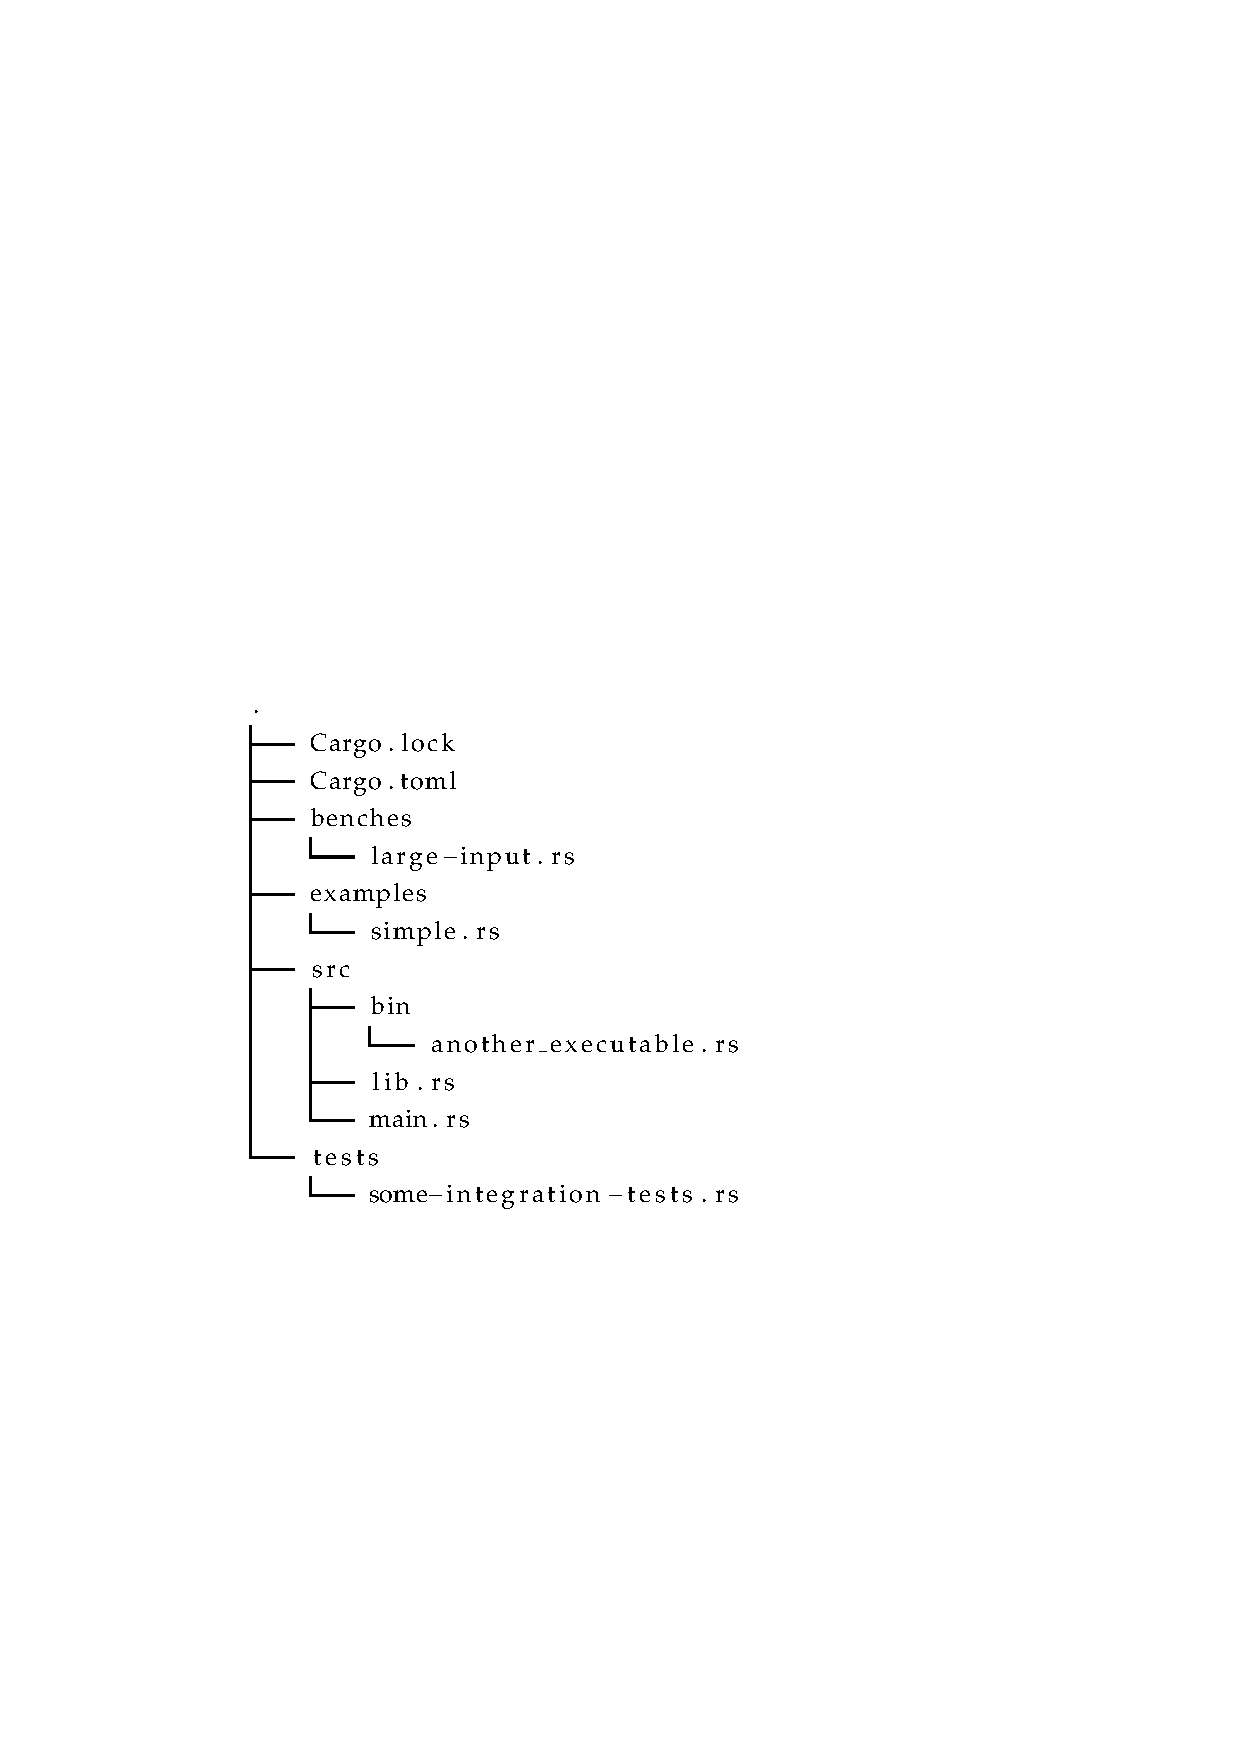
\includegraphics{Toolchain/dateibaum.pdf}
    \caption{Dateibaum eines Rust Projekts}
\end{figure}

\begin{itemize}
    \item Cargo.toml und Cargo.lock werden im Wurzelverzeichnis des Projekts gespeichert
    \item Quellcode-Dateien sind im src-Ordner vorgesehen
    \item Die Standarddatei für Bibliotheken ist src/lib.rs
    \item Die Standarddatei für ausführbare Programme ist src/main.rs
    \item Quellcode für sekundäre ausführbare Programme src/bin/*.rs
    \item Integrationstests im Ordner tests, Unit-Tests werden in die jeweilige Programmdatei geschrieben
    \item Beispiele im examples Ordner
    \item Benchmarks im benches Ordner
\end{itemize}

\subsubsection{Wichtige Kommandozeilenbefehle für Cargo}

Zum Kompilieren uns Ausführen:

\begin{lstlisting}
    $ cargo build
    $ ./target/debug/hello_world

    $ cargo build --release             # optimized performance
    $ ./target/release/hello_world

    # alternative as one command
    $ cargo run
\end{lstlisting}

Zum Testen:

\begin{lstlisting}
    # run all standard tests
    $ cargo test

    # run all tests marked as ignored
    $ cargo test -- --ignored
\end{lstlisting}

\subsection{Veröffentlichung bei crates.io}

Das Paketeregister der Rust-Community, genannt crates.io, ist ein Ort für Bibliotheken, die von verschiedenen Programmierern aus der Community verwaltet werden. Eine Veröffentlichung ist permanent. Das heißt, dass keine Versionsnummern überschrieben werden können und somit der Code nicht gelöscht werden kann. Jedoch gibt es keine Begrenzung für die Anzahl der Versionen, die veröffentlicht werden können.

Vor der Veröffentlichung wird ein Account benötigt. Dazu muss mit einem Github-Account auf crates.io ein API-Token generiert werden. Danach kann man sich über einen Befehl auf der Kommandozeile anmelden:

\begin{lstlisting}
    $ cargo login abcdefghijklmnopqrstuvwxyz012345
\end{lstlisting}

Dieser Token wird anschließend in einem lokalen Verzeichnis gespeichert und sollte nicht mit anderen geteilt werden. Erneute Generierung eines Tokens ist möglich.

Mithilfe von Cargo werden eigene Bibliotheken paketiert, dabei entsteht eine *.crate-Datei im Unterverzeichnis target/package.

\begin{lstlisting}
    $ cargo package
\end{lstlisting}

Dabei ist zu beachten, dass es eine Beschränkung der Uploadgröße von 10 MB für *.crate-Dateien gibt. Um die Dateigröße einzuschränken, können Dateien exkludiert bzw. inkludiert werden, dazu stehen die Schlüsselwörter \glqq exclude\grqq{} (blacklisting) und \glqq include\grqq{} (whitelisting) in der Cargo.toml-Datei zur Verfügung:

\begin{lstlisting}
    [package]
    # ...
    exclude = [
        "public/assets/*",
        "videos/*",
    ]
\end{lstlisting}

bzw.

\begin{lstlisting}
    [package]
    # ...
    include = [
        "**/*.rs",
        "Cargo.toml",
    ]
\end{lstlisting}

Zu beachten ist, dass das Schlüsselwort \glqq include\grqq{}, wenn gesetzt, \glqq exclude\grqq{} überschreibt.

Zum Hochladen muss nur noch folgender Befehl ausgeführt werden:

\begin{lstlisting}
    $ cargo publish
\end{lstlisting}

Dieser Befehl paketiert die Bibliothek automatisch, falls keine lokale crate-Datei gefunden wurde.

Zum Veröffentlichen einer neuen Version muss lediglich die Versionsnummer in der Cargo.toml verändert werden.

\subsubsection{Verwalten eines crate.io basierten Pakets}

Die Verwaltung eines Pakets geschieht in Rust primär auf der Kommandozeilenebene mit Cargo.

Wenn ein schwerwiegender Bug in einem bereits hochgeladenen Paket gefunden wurde, kann diese Version aus dem Index von crates.io entfernt, jedoch nicht gelöscht werden.

\begin{lstlisting}
    $ cargo yank --vers 1.0.1
    $ cargo yank --vers 1.0.1 --undo    # undo the yank
\end{lstlisting}

Diese Pakete können immer noch heruntergeladen und in andere Projekte eingebunden werden, die bereits an \glqq yanked\grqq{} Pakete gebunden waren. Cargo lässt dies dies nicht bei neu erstellten Crates\footnote{Bibliothek oder Paket in Rust} zu.

Ein Projekt wird meist von mehreren Entwicklern programmiert oder Besitzer des Projekts ändert sich im Laufe der Zeit. Folgende Befehle fügen neue Entwickler zu einem Projekt hinzu, welche dann in der Lage sind, auf crates.io zu veröffentlichen bzw. entfernen sie aus dem Projekt:

\begin{lstlisting}
    # "named" owner:
    $ cargo owner --add my-buddy
    $ cargo owner --remove my-buddy

    # "team" owner:
    # syntax: github:org:team
    $ cargo owner --add github:rust-lang:owners
    $ cargo owner --remove github:rust-lang:owners
\end{lstlisting}

Wenn ein Teamname angegeben wird, sind diese nicht befugt, neue \glqq owner\grqq{} hinzuzufügen. Die Befehle yank und publish sind Teams jedoch erlaubt. Ist ein \glqq named owner\grqq{} in einem Team, so sind alle Entwickler eines Teams als \glqq named owner\grqq{} eingestuft.

\subsection{Externe Tools}

Cargo versucht, die Integration von Tools von Drittanbietern zu vereinfachen, z.B. für IDEs oder anderen Build-Systemen. Dazu verfügt Cargo über mehrere Möglichkeiten:

\begin{itemize}
    \item cargo metadata-Befehl
    \item message-format Argument
    \item benutzerdefinierte Befehle
\end{itemize}

\subsubsection{Information über die Paketstruktur mit cargo metadata}

\begin{lstlisting}
    $ cargo metadata
\end{lstlisting}

Dieser Befehl gibt im JSON-Format alle Metadaten über ein Projekt aus. Darunter Befinden sich die Version des aktuellen Projekts sowie eine Liste der Pakete und Abhängigkeiten. Grobe Struktur:

\begin{lstlisting}
    {
        "version": integer,
        "packages": [ {
            "id": PackageId,
            "name": string,
            "version": string,
            "source": SourceId,
            "dependencies": [ Dependency ],
            "targets": [ Target ],
            "manifest_path": string,
        } ],
        "workspace_members": [ PackageId ],
        "resolve": {
            "nodes": [ {
                "id": PackageId,
                "dependencies": [ PackageId ]
            } ]
        }
    }
\end{lstlisting}

\subsubsection{Informationen beim Kompilieren}

Mit dem Argument \glqq message-format\grqq{} können genauere Informationen beim Kompilieren herausgefiltert werden:

\begin{lstlisting}
    $ cargo build --message-format=json
\end{lstlisting}

Dadurch entsteht ein Output im JSON-Format mit Informationen über Compiler-Fehlermeldungen und -Warnungen, erzeugte Artefakte und das Ergebnis.

\subsubsection{Benutzerdefinierte Befehle}

Cargo ist so ausgelegt, dass es erweitert werden kann, ohne dass Cargo selbst modifiziert werden muss. Dazu muss ein Programm in der Form cargo-\textit{command} in einem der \$PATH-Verzeichnisse des Benutzers liegen. Anschließend kann es von Cargo aufgerufen werden mit \glqq cargo \textit{command}\grqq{}.Wenn ein solches Programm von Cargo aufgerufen wird, übergibt es, wie es üblich ist, als ersten Parameter den Programmnamen. Als zweites die Bezeichnung des Programms (\textit{command}). Alle weiteren Parameter in der Befehlszeile werden unverändert weitergeleitet.

Beispiel:

\begin{lstlisting}
    // cargo-listargs
    use std::env;

    fn main() {
        let args: Vec<_> = env::args().collect();
        println!("{:?}", args);
    }
\end{lstlisting}

Obiges Programm gibt eine Liste der Parameter aus, die übergeben wurden. Es könnte auch in C programmiert sein, entscheidend ist, dass der Programmname in der richtigen Form ist.

\begin{lstlisting}
    $ ./cargo-listargs arg1 arg2
    # ["./cargo-listargs", "arg1", "arg2"]

    $ cargo listargs arg1 arg2
    # ["path/to/cargo-listargs", "listargs", "arg1", "arg2"]
\end{lstlisting}

Im Internet gibt es zum Zeitpunkt der Erstellung dieses Dokuments bereits über 40 benutzerdefinierte Befehle, die von der Rust-Community erstellt wurden. \cite{CargoSubcommands}

\chapter{Programmierung mit Rust und Unterschiede zu C/C++}

In diesem Kapitel werden auf Unterschiede bei der Programmierung zwischen den Sprachen Rust und C/C++ eingegangen.


\section{Grundlagen}

Zu den Grundlagen einer jeden Programmiersprache gehört der Umgang mit Variablen und Datentypen, und Kommentarfunktionen. Kontrollstrukturen definieren die Reihenfolge, in der Berechnungen durchgeführt werden.

\subsection{Variablen und Mutabilität}

In Rust sind Variablen standardmäßig unveränderlich. Das ist einer von vielen Faktoren, die Programmierer helfen sollen, den Code so zu schreiben, dass die Sicherheit und Parallelität von Rust genutzt werden. \cite{RustBook}

Ein Beispiel in Rust:

\begin{lstlisting}
    fn main() {
        let x = 5;
        println!("The value of x is {}", x);
        x = 6;
        println!("The value of x is {}", x);
    }
\end{lstlisting}

Beim Kompilieren erscheint folgende Fehlermeldung:

\begin{lstlisting}
    error[E0384]: cannot assign twice to immutable variable 
    `x`
    --> src/main.rs:4:5
     |
   2 |     let x = 5;
     |         -
     |         |
     |         first assignment to `x`
     |         help: make this binding mutable: `mut x`
   3 |     println!("The value of x is {}", x);
   4 |     x = 6;
     |     ^^^^^ cannot assign twice to immutable variable
   
\end{lstlisting}

Das Beispiel zeigt, wie der Compiler dem Programmierer hilft, Fehler im Programm zu finden. Die Fehlermeldung weist darauf hin, dass die Fehlerursache darin liegt, dass auf eine unveränderliche Variable nicht ein zweites Mal zugewiesen werden darf.

Bei C oder C++ ist jede Variablendefinition standardmäßig veränderlich, das heißt bei gleicher Vorangehensweise würde folgendes C-Programm ohne Fehlermeldungen übersetzen:

\begin{lstlisting}
    #include <stdio.h>

    int main()
    {
        int x = 5;
        printf("The value of x is %d\n", x);
        x = 6;
        printf("The value of x is %d\n", x);
        return 0;
    }    
\end{lstlisting}

Das Schlüsselwort \verb"const" kann verwendet werden, um Variablen in C/C++ konstant zu definieren.

\begin{lstlisting}
    const int x = 5;
\end{lstlisting}

Wird in C versucht, eine konstant definierte Variable zu verändern, indem ein Wert mit einem nicht konstanten Typ verwendet wird, ist das Verhalten nicht definiert. \cite[p.~87]{ISO:9899:2017}

Das Verhalten in Folgendem Beispiel ist somit nicht definiert:

\begin{lstlisting}
    #include <stdio.h>

    int main()
    {
        const int x = 5;
        printf("The value of x is %d\n", x);
        *(int *)&x = 6;
        printf("The value of x is %d\n", x);
        return 0;
    }
\end{lstlisting}

Ergebnis mit dem Clang Compiler in der Version 7.0.1 auf einem Linux System (keine Warnungen beim Kompilieren):

\begin{lstlisting}
    The value of x is 5
    The value of x is 5
\end{lstlisting}

Ergebnis mit dem GCC Compiler in der Version 8.3.1 auf einem Linux System (auch hier keine Warnungen):

\begin{lstlisting}
    The value of x is 5
    The value of x is 6
\end{lstlisting}

\subsection{Datentypen}\label{chap:datatypes}

Jede Variable in Rust hat einen bestimmten Datentyp. In Rust wird unterschieden zwischen skalaren und zusammengesetzten Typen. Rust ist eine statisch typisierte Sprache. Das bedeutet, dass die Typen aller Variablen zur Kompilierzeit bekannt sein müssen. Der Compiler kann normalerweise ableiten, welcher Typ verwenden soll, basierend auf dem Wert und wie er verwendet wird. In Fällen, in denen viele Typen möglich sind, z.B. wenn ein String in einen numerischen Typ konvertiert werden soll, muss eine Typanmerkung wie folgt hinzugefügt werden:

\begin{lstlisting}
    let guess: u32 = "42".parse().expect("Not a number!");
\end{lstlisting}

Ohne Angabe des Typs gibt der Rust-Compiler eine Fehlermeldung aus.

\subsubsection{Integer Typ}

Ein Integer ist ein Datentyp für ganze Zahlen. Der Typ \verb"u32" gibt an, dass es sich um eine vorzeichenlose Ganzzahl handelt, vorzeichenbehaftete Ganzzahltypen beginnen mit \glqq i\grqq{} an Stelle von \glqq u\grqq{}. Due Zahl gibt an, wie viel Speicherplatz sie beansprucht. Folgende Tabelle zeigt die Integertypen von Rust und C:

\begin{table}[htbp]
\centering
\begin{tabular}{|c||c|c||c|c|}
\hline
\rule[-1ex]{0pt}{2.5ex} & \multicolumn{2}{|c||}{Rust} & \multicolumn{2}{|c|}{C/C++} \\
\hline
\rule[-1ex]{0pt}{2.5ex} Länge & signed & unsigned & signed & unsigned \\
\hline
\rule[-1ex]{0pt}{2.5ex} 8-bit & i8 & u8 & \_\_int8\_t & \_\_uint8\_t \\
\hline
\rule[-1ex]{0pt}{2.5ex} 16-bit & i16 & u16 & \_\_int16\_t & \_\_uint16\_t \\
\hline
\rule[-1ex]{0pt}{2.5ex} 32-bit & i32 & u32 & \_\_int32\_t & \_\_uint32\_t \\
\hline
\rule[-1ex]{0pt}{2.5ex} 64-bit & i64 & u64 & \_\_int64\_t & \_\_uint64\_t \\
\hline
\rule[-1ex]{0pt}{2.5ex} 128-bit & i128 & u128 & \_\_int128\_t & \_\_uint128\_t \\
\hline
\rule[-1ex]{0pt}{2.5ex} arch & isize & usize & & \\
\hline
\end{tabular}
\caption{Integertypen in Rust und C/C++}
\end{table}

Mit \verb"short" und \verb"long" sollen verschieden lange ganzzahlige Werte zur Verfügung stehen, soweit dies praktikabel ist; \verb"int" wird normalerweise die natürliche Größe für eine bestimmte Maschine sein. \verb"short" belegt oft 16 Bits, \verb"long" 32 Bits und \verb"int" entweder 16 oder 32 Bits. Es steht jedem Übersetzer frei, sinnvolle Größen für seine Maschine zu wählen, nur mit den Einschränkungen, dass \verb"short" und \verb"int" wenigstens 16 Bits haben, \verb"long" mindestens 32 Bits, und dass \verb"short" nicht länger als \verb"int" und \verb"int" nicht länger als \verb"long" sein darf. \cite{ProgInC}

Beispiel:

\begin{lstlisting}
    printf("%zu\n", sizeof(char));      // 1:  8-bit
    printf("%zu\n", sizeof(short));     // 2: 16-bit
    printf("%zu\n", sizeof(int));       // 4: 32-bit
    printf("%zu\n", sizeof(long));      // 8: 64-bit
\end{lstlisting}

In Rust hängen die Typen \verb"isize" und \verb"usize" von der Art des Computers ab, auf dem das Programm ausgeführt wird: 64 Bits bei 64-Bit-Architektur und 32 Bits bei 32-Bit-Architektur.

In Rust wird standardmäßig der Integertyp i32 verwendet. Dieser Typ ist im Allgemein der schnellste Typ, auch auf 64-Bit-Systemen. Die Typen \verb"isize" und \verb"usize" können zum indexieren von Arrays verwendet werden.

\subsubsection{Weitere Typen in Rust}

\begin{itemize}
    \item Fließkomma-Typen: \verb"f32" und \verb"f64" (Standard ist \verb"f64")
    \item Boolean: \verb"bool" true / false
    \item Zeichentyp \verb"char": Unicode, das heißt chinesische, japanische und koreanische Zeichen, Emoji, Leerzeichen mit Nullbreite sind möglich
\end{itemize}

\subsubsection{Tupel}

Ein Tupel ist ein allgemeiner Weg, um einige andere Werte mit verschiedenen Typen zu einem Verbindungstyp zu gruppieren. Tupel haben eine feste Länge, das heißt sie können nicht größer oder kleiner werden nachdem sie deklariert wurden.

\begin{lstlisting}
    fn main() {
        let tup: (i32, f64, u8) = (500, 6.4, 1);
        let (x, y, z) = tup;
        println!("The value of y is: {}", y);
        println!("The value of z is: {}", tup.2);
    }
\end{lstlisting}

\subsubsection{Arrays}

Eine andere Möglichkeit, eine Sammlung mehrerer Werte zu haben, besteht in einem Array. Im Gegensatz zu einem Tupel muss jedes Element eines Arrays denselben Typ haben. Arrays in Rust unterscheiden sich von Arrays in einigen anderen Sprachen, da Arrays in Rust eine feste Länge haben, wie Tupel.

In Rust werden die Werte, die in ein Array gehen, als durch Kommata getrennte Liste in eckiggen Klammern geschrieben:

\begin{lstlisting}
    let a = [1, 2, 3, 4, 5];
\end{lstlisting}

Arrays sind nützlich, um Daten auf dem Stack statt auf dem Heap zuweisen zu können oder um sicherzustellen, dass immer eine feste Anzahl von Elementen vorhanden sind. Ein Array ist jedoch nicht so flexibel wie der Vektortyp. Ein Vektor ist ein ähnlicher Auflistungstyp, der von der Standardbibliothek bereitgestellt wird und dessen Größe vergrößert oder verkleinert werden darf.

Das Schreiben des Array-Typs erfolgt mit eckigen Klammern mit dem Typ der Element im Array gefolgt von einem Semikolon und die Anzahl der Elemente im Array:

\begin{lstlisting}
    let a: [i32; 5] = [1, 2, 3, 4, 5];
\end{lstlisting}

Eine ähnliche Schreibweise wird zum Initialisieren eines Arrays verwendet, das für jedes Element den selben Wert enthält. Dabei wird der Anfangswert, dann ein Semikolon und die Länge des Array angegeben:

\begin{lstlisting}
    let a = [3; 5];
\end{lstlisting}

Das Array mit dem Namen \glqq a\grqq{} enthält 5 Elemente, die zunächst alle auf den Wert 3 gesetzt sind. Folgender Ausdruck erzeugt das gleiche Array:

\begin{lstlisting}
    let a = [3, 3, 3, 3, 3];
\end{lstlisting}

Ein Array ist ein einzelner Speicherbereich, der auf dem Stack reserviert ist. Es kann mithilfe der Indexierung wiefolgt zugegriffen werden:

\begin{lstlisting}
    let a = [1, 2, 3, 4, 5];
    let first = a[0];
    let second = a[1];
\end{lstlisting}

Wird auf ein Element zugegriffen, das nicht innerhalb des Bereichs ist, beendet sich das Programm mit folgender Meldung:

\begin{lstlisting}
    thread 'main' panicked at 'index out of bounds: the len
    is 5 but the index is 10', src/main.rs:5:13
    note: Run with `RUST_BACKTRACE=1` environment variable
    to display a backtrace.
\end{lstlisting}

Wenn in C oder C++ auf ein Element außerhalb des Bereichs eines Arrays zugegriffen wird, fällt dies beim Testen wesentlich weniger auf, da normalerweise das Programm weiter ausgeführt wird.

Das ist ein Beispiel der Sicherheitsprinzipien von Rust. Viele Low-Level-Pro\-gram\-mier\-spra\-chen verzichten auf diesen Check, sodass ein ungültiger Speicherbereich indexiert werden kann. Rust verhindert dies durch sofortiges Beenden des Programms.

\subsection{Funktionen}

In Rust werden Funktionen und Variablennamen als Konvention in snake case geschrieben. Ein Programm, das eine Beispielfunktion enthält:

\begin{lstlisting}
    fn main() {
        println!("Hello, world!");
        another_function(42);
    }
    fn another_function(n: i32) {
        println!("Another function with number {}.", n);
    }
\end{lstlisting}

Eine Funktion mit Parameter enthält den Namen der Variable sowie den Typen mit einem Doppelpunkt getrennt. Bei mehreren Parametern werden diese durch Komma getrennt.

Bei Funktionen mit Rückgabewerten muss am Ende des Funktionskörpers der Rückgabewert als Expression ohne Semikolon stehen. Wenn eine Funktion früh beendet werden soll, kann ein \verb"return" mit Rückgabewert benutzt werden. Der Rückgabetyp der Funktion muss mit einem Pfeil(\verb"->") angegeben werden.

\begin{lstlisting}
    fn main() {
        let result = add(12, 34);
        println!("The result is {}.", result);
    }
    fn add(n1: i32, n2: i32) -> i32 {
        n1 + n2
    }
\end{lstlisting}

\subsection{Kontrollstrukturen}

Kontrollstrukturen definieren die Reihenfolge, in der Berechnungen durchgeführt werden. Die Entscheidung, ob Code ausgeführt werden soll oder nicht, abhängig davon, ob eine Bedingung wahr ist, und die Entscheidung, wiederholt Code aus\-zu\-füh\-ren, während eine Bedingung wahr ist, sind grundlegende Bausteine in den meisten Programmiersprachen. Die häufigsten Konstrukte, mit denen der Ausführungsfluss von Rust-Code gesteuert werden kann, sind \verb"if"-Ausdrücke und -Schleifen.

\subsubsection{\texttt{if}-Anweisungen}

Mit \verb"if"-\verb"else"-Anweisungen werden Entscheidungen formuliert. Der else-Teil ist optional. Beispiel:

\begin{lstlisting}
    if number < 5 {
        println!("condition was true");
    } else {
        println!("condition was false");
    }
\end{lstlisting}

Diese Anweisungen sind syntaktisch wie in C oder C++, mit dem Unterschied, dass keine Klammern bei der Expression benötigt werden.

In Rust muss der Typ der Expression ein Boolean sein. Folgendes Programm wird also nicht übersetzt:

\begin{lstlisting}
    fn main() {
        let number = 3;
        if number {                     // type must be bool
            println!("number was three");
        }
    }
\end{lstlisting}

C und C++ prüfen bei einer \verb"if"-Anweisung mit einem Integer Wert nur, ob dieser den Wert 0 hat. Da in Rust ein Boolean Typ benötigt wird, muss das Programm umgeschrieben werden:

\begin{lstlisting}
    fn main() {
        let number = 3;
        if number != 0 {
            println!("number was something other than 0");
        }
    }
\end{lstlisting}

Mehrere Bedingungen können auch in Rust in einer \verb"else if"-Anweisung behandelt werden:

\begin{lstlisting}
    let number = 6;

    if number % 4 == 0 {
        println!("number is divisible by 4");
    } else if number % 3 == 0 {
        println!("number is divisible by 3");
    } else if number % 2 == 0 {
        println!("number is divisible by 2");
    } else {
        println!("number is not divisible by 4, 3, or 2");
    }
\end{lstlisting}

In Rust ist die \verb"if"-Anweisung eine Expression, somit kann es verwendet werden, um z.B. Werte von Variablen zu definieren:

\begin{lstlisting}
    let condition = true;
    let number = if condition {
        5
    } else {
        6
    };
\end{lstlisting}

Da Rust eine statisch typisierte Sprache ist, muss der Typ beim Kompilieren bekannt sein. Das heißt, dass bei letzteren \verb"if"-Anweisung der Typ einheitlich sein muss. Im letzten Beispiel war \verb"number" vom Typ \verb"i32".

\subsubsection{Schleifen}

Rust hat drei Arten von Schleifen: loop, while und for.

Loop-Schleifen führen Code so oft aus, bis sie explizit gestoppt werden mit dem Schlüsselwort \verb"break". Schleifen können in Rust auch als Expression verwendet werden, wenn an dem \verb"break" ein Wert angefügt wird:

\begin{lstlisting}
    fn main() {
        let mut counter = 0;
        let result = loop {
            counter += 1;
            if counter == 10 {
                break counter * 2;      // loop returning 20
            }
        };
        println!("The result is {}", result);
    }
\end{lstlisting}

\verb"while"-Schleifen gibt es auch in C und C++. Sie funktionieren auch in Rust entsprechend.

\begin{lstlisting}
    fn main() {
        let a = [10, 20, 30, 40, 50];
        let mut index = 0;
        while index < 5 {
            println!("the value is: {}", a[index]);
            index = index + 1;
        }
    }
\end{lstlisting}

Das Programm gibt alle Werte aus dem Array aus. Alternativ kann hier mit einer \verb"for"-Schleife gearbeitet werden. For-Schleifen funktionieren in Rust anders als in C oder C++, sie gleichen ehr einer \verb"for"-\verb"each"-Schleife aus Java. Das heißt, dass der Code für jedes Element aus einer Sammlung einmal ausgeführt wird.

\begin{lstlisting}
    fn main() {
        let a = [10, 20, 30, 40, 50];
        for element in a.iter() {
            println!("the value is: {}", element);
        }
    }
\end{lstlisting}

Mit \verb"for"-Schleifen kann in Rust die Sicherheit des Codes erhöht werden, da dadurch Zugriffe außerhalb eines Arrays verhindert werden.


\section{Ownership}

Ownership ist ein einzigartiges Merkmal von Rust. Es ermöglicht Speichersicherheit zur Kompilierzeit ohne die Notwendigkeit eines Garbage Collectors. Daher ist es wichtig, das Ownership-Prinzip als Programmierer zu verstehen. In diesem Kapitel wird Ownership und damit zusammenhängende Eigenschaften wie Borrowing, Slices und wie Rust Daten im Arbeitsspeicher ablegt beschrieben.

\subsection{Funktionsweise von Ownership}

Alle Computerprogramme müssen Arbeitsspeichermanagement betreiben. Man\-che Sprachen benutzen einen Garbage Collector, welcher währen der Programmlaufzeit nach nicht mehr benutzten Speicher sucht und diesen frei gibt. In andern Sprachen muss der Programmierer explizit Speicher zuweisen und freigeben. Rust geht anders vor: Speicher wird durch ein System von Besitz und einen Satz an Regeln gestützt, welches der Compiler zur Kompilierzeit überprüft, sodass das Programm zur Laufzeit nicht gebremst wird.

\subsubsection{Regeln}

\begin{itemize}
    \item Jeder Wert in Rust hat eine Variable, die als Eigentümer bezeichnet wird.
    \item Es kann immer nur ein Besitzer gleichzeitig sein.
    \item Wenn der Besitzer den Gültigkeitsbereich verlässt, wird der Wert gelöscht.
\end{itemize}

\subsubsection{Beispiel: String}

Um die Eigentumsregeln zu veranschaulichen, ist ein komplexerer Datentyp not\-wen\-dig als die, die in \autoref{chap:datatypes} behandelt wurden, denn diese werden auf dem Stack gespeichert. In diesem Beispiel sollen Daten, die auf dem Heap gespeichert werden, betrachtet werden um zu veranschaulichen, wie Rust weiß, wann diese Daten zu bereinigen sind. Hierfür wird im Folgenden der Typ \verb"String" verwendet. Diese Aspekte gelten auch für andere komplexe Datentypen, die von der Standardbibliothek bereitgestellt werden.

Wenn ein Rust-Programm eine Eingabe von einem Benutzer speichern möchte, muss ein Datentyp verwendet werden, welche eine variable Länge haben kann. Einen solchen String kann man in Rust zum Beispiel mit der \verb"from"-Funktion erstellen:

\begin{lstlisting}
    let mut s = String::from("hello");
    s.push_str(", world!");             // appends a literal
    println!("{}", s);                  // 'hello, world!'
\end{lstlisting}

Um einen veränderlichen String zu erzeugen, muss Speicherplatz auf dem Heap zugewiesen werden, welcher zu Kompilierzeit unbekannt ist. Das heißt:

\begin{enumerate}
    \item Speicherplatz muss vom Betriebssystem zur Laufzeit bereitgestellt werden.
    \item Der Speicherplatz muss wieder freigegeben werden, wenn der String nicht mehr benötigt wird.
\end{enumerate}

Der erste Teil wird manuell vom Programmierer initiiert, beim Aufruf von \verb"String::from".

Der zweite Teil geschieht automatisch (durch die Methode \verb"drop"), sobald die Variable, die es besitzt, den Gültigkeitsbereich verlässt, zum Beispiel am Ende des Blocks.

\begin{lstlisting}
    {
        let s = String::from("hello");
        // s is valid from this point forward
    
        // doo stuff with s
    }                    // this scope is neo over, and s is
                         // no longer valid
\end{lstlisting}

In C++ wird dieses Muster der Freigabe von Ressourcen am Ende der Lebensdauer eines Elements manchmal als \textit{Ressourcenbelegung ist Initialisierung (Resource Acquisition Is Initialization, kurz RAII)} bezeichnet. \cite[p.~71]{CppProg}

Dieses Muster hat einen tiefgründigen Einfluss auf die Schreibweise von Rust-Code. Es mag einfach erscheinen, aber das Verhalten von Code kann in komplizierten Situationen unerwartet sein, wenn mehrere Variablen die Daten verwenden sollen, die auf dem Heap zugewiesen wurden.

\subsubsection{Variablen und Daten: Move}

Mehrere Variablen können in Rust auf unterschiedliche Weise mit denselben Daten interagieren. Ein Beispiel mit Integer:

\begin{lstlisting}
    let x = 5;
    let y = x;
\end{lstlisting}

Hier wird der Wert 5 an die Variable \verb"x" gebunden und anschließend eine Kopie von \verb"x" an die Variable \verb"y" gebunden. Denn Integer haben eine feste Größe im Speicher und können auf dem Stack gespeichert werden.

Beispiel mit String:

\begin{lstlisting}
    let s1 = String::from("hello");
    let s2 = s1;
\end{lstlisting}

Dies sieht dem vorherigen Code sehr ähnlich, aber die Funktionsweise ist nicht dieselbe, denn Strings werden in Rust im Heap gespeichert.

\begin{figure}[htbp]
    \centering
    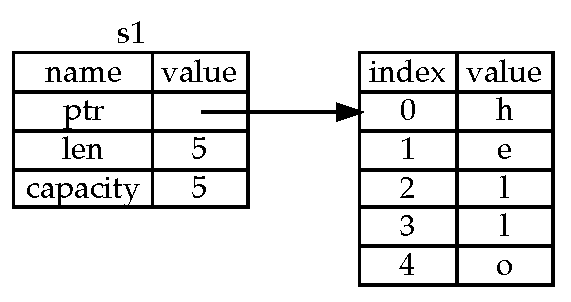
\includegraphics[scale=0.9]{Programmierung/Tabelle1.pdf}
    \caption{Repräsentation des Speichers eines String}
    \label{fig:tabelle1}
\end{figure}

\autoref{fig:tabelle1} zeigt die Bestandteile von String. Er besteht aus drei Teilen, zu sehen in der linken Tabelle: einen Pointer auf den Speicher, der den String enthält, die Länge und die Kapazität. Diese Datengruppe wird auf dem Stack gespeichert. Auf der rechten Seite befindet sich der Speicher auf dem Heap, der den Inhalt enthält.

Bei der Zuweisung von \verb"s1" zu \verb"s2" werden nur die String-Daten kopiert, das heißt der Pointer, die Länge und die Kapazität, welche sich auf dem Stack befinden. Die Daten des Heaps werden nicht kopiert.

\begin{figure}[htbp]
    \centering
    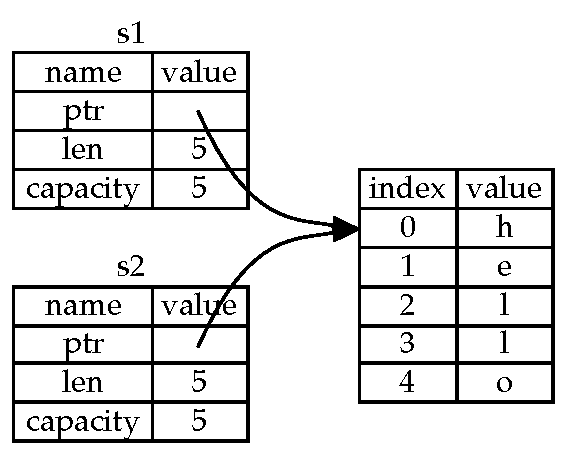
\includegraphics[scale=0.9]{Programmierung/Tabelle2.pdf}
    \caption{Repräsentation des Speichers eines String: Kopie auf dem Stack}
    \label{fig:tabelle2}
\end{figure}

Wenn Rust eine vollständige Kopie gemacht hätte, würden die Daten wie auf \autoref{fig:tabelle3} aussehen. Und die Operation \verb"s2 = s1" kann hinsichtlich der Lauf\-zeit\-leis\-tung sehr euer sein, wenn die Daten auf dem Heap groß wären.

\begin{figure}[htbp]
    \centering
    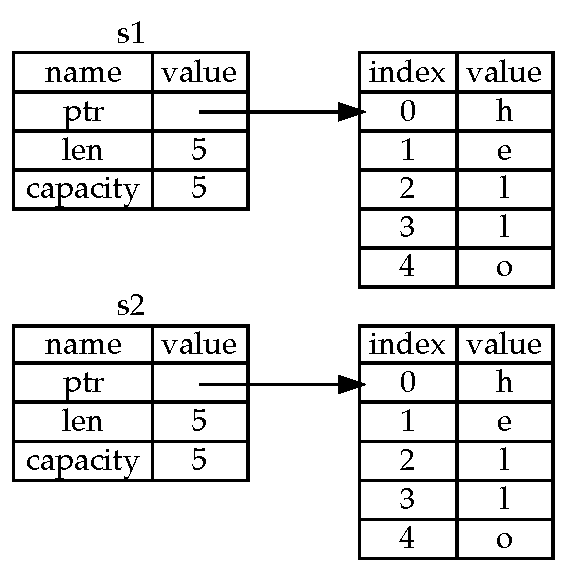
\includegraphics[scale=0.9]{Programmierung/Tabelle3.pdf}
    \caption{Repräsentation des Speichers eines String: Vollständige Kopie}
    \label{fig:tabelle3}
\end{figure}

Sobald eine Variable außerhalb des Gültigkeitsbereichs gelangt, wird der Spei\-cher aus dem Heap gelöscht. Aber da \autoref{fig:tabelle2} zwei Variablen zeigt, die auf den selben Speicherbereich im Heap zeigen, würde zwei mal der Speicherbereich freigegeben werden. Das ist bekannt als \glqq double free\grqq{}-Error und kann zu Speicherbeschädigungen und möglicherweise zu Sicherheitsanfälligkeiten führen.

Um die Speichersicherheit zu gewährleisten, hält Rust \verb"s1" für ungültig und muss somit nichts löschen, wenn \verb"s1" den Gültigkeitsbereich verlässt.

Das hat zu Folge, dass \verb"s1" nicht mehr genutzt werden kann, nachdem es \verb"s2" zugewiesen wurde:

\begin{lstlisting}
    let s1 = String::From("hello");
    let s2 = s1;

    println!("{}, world!", s1);
\end{lstlisting}

Daraus entsteht folgende Fehlermeldung:


\begin{lstlisting}
    error[E0382]: borrow of moved value: `s1`
     --> src/main.rs:5:28
      |
    3 |     let s1 = String::from("hello");
      |         -- move occurs because `s1` has type
    `std::string::String`, which does not implement the
    `Copy` trait
    4 |     let s2 = s1;
      |              -- value moved here
    5 |     println!("{}, world!", s1);
      |                            ^^ value borrowed here
    after move
\end{lstlisting}

Diese Art von Kopieren, welche die erste Variable ungültig macht, nennt man in Rust \glqq move\grqq{} (\verb"s1" was \textit{moved} into \verb"s2"). Was also tatsächlich passiert, wird in \autoref{fig:tabelle4} dargestellt.

\begin{figure}[htbp]
    \centering
    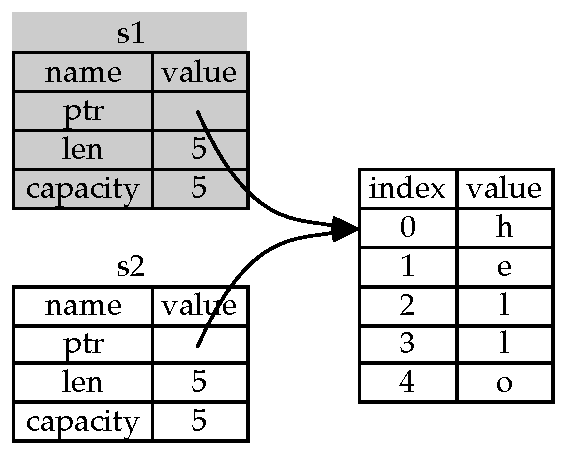
\includegraphics[scale=0.9]{Programmierung/Tabelle4.pdf}
    \caption{Repräsentation des Speichers eines String: Moved}
    \label{fig:tabelle4}
\end{figure}

Somit gibt es keinen \glqq double free\grqq{}-Error, da der Speicher nur einmal freigegeben wird, wenn \verb"s2" den Gültigkeitsbereich verlässt.

\subsubsection{Variablen und Daten: Clone}

Wenn eine vollständige Kopie erstellt werden soll, kann die Methode \verb"clone" benutzt werden. Beispiel:

\begin{lstlisting}
    let s1 = String::from("hello");
    let s2 = s1.clone();

    println!("s1 = {}, s2 = {}", s1, s2);
\end{lstlisting}

Der Code kompiliert ohne Fehlermeldungen und erzeugt explizit das in \autoref{fig:tabelle3} gezeigte Verhalten, bei dem die Heap-Daten kopiert werden.

\subsubsection{Stack-Only-Daten kopieren}

Primitive Datentypen, die komplett auf dem Stack gespeichert sind, können nicht übergeben werden (Move nicht möglich), sie können nur vollständige kopiert werden. Darum würde folgender Code ohne Fehler übersetzen:

\begin{lstlisting}
    let x = 5;
    let y = x;

    println!("x = {}, y = {}", x, y);
\end{lstlisting}

Integer besitzen eine feste Speichergröße zur Kompilierzeit. Es macht keinen Unterschied, sie mit \verb"clone" zu kopieren. Wenn ein Typ den \verb"Copy"-Trait besitzt, kann die erste Variable nach der Zuweisung weiter verwendet werden. In der Regel kann jede Gruppe einfacher Skalarwerte über den Stack vollständig kopiert werden. Einige der Typen sind:

\begin{itemize}
    \item Alle Integer-Typen, z.B. \verb"u32"
    \item Boolean-Typ, \verb"bool" mit den Werten \verb"true" und \verb"false"
    \item Alle Fließkommazahlen wie z.B. \verb"f64"
    \item Zeichentyp \verb"char"
    \item Tupel, wenn sie nur Typen beinhalten, die den \verb"Copy"-Trait implementieren z.B. \verb"(i32, i32)", jedoch nicht \verb"(i32, String)"
\end{itemize}

\subsubsection{Ownership und Funktionen}

Die Semantik für die Übergabe eines Wertes an eine Funktion ähnelt derjenigen, die einer Variablen einen Wert zuweist. Das Übergeben einer Variablen an einer Funktion wird genauso wie die Zuweisung verschoben oder kopiert. Folgendes Programm enthält ein Beispiel mit einigen Anmerkungen, die zeigen, wo Variablen in den Geltungsbereich gelangen und aus diesem Bereich herauskommen:

\begin{lstlisting}
    fn main() {
        let s = String::from("hello");  // s comes
                                        // into scope
        takes_ownership(s);         // s's value moved into
                                    // the function...
        // ... and is no longer valid here

        let x = 5;         // x comes into scope

        makes_copy(x);     // x would move into the function
                           // but i32 is Copy, so it's okay
                           // to still use x afterward

    } // Here, x goes out of scope, then s. But because s's
      // value was moved, nothing special happens.


    fn takes_ownership(some_string: String) {
        // some_string comes into scope

        println!("{}", some_string);
    } // Here, some_string goes out of scope and 'drop' is
      // called. The backing memory is freed.


    fn makes_copy(some_integer: i32) {
        // some_integer comes into scope

        println!("{}", some_integer);
    } // Here, some_integer goes out of scope. Nothing
      // special happens.
\end{lstlisting}

Wenn \verb"s" nach der Methode \verb"takes_ownership" genutzt wird, würde Rust einen Fehler bei der Kompilierung ausgeben. Diese statischen Checks sollen Fehler im Programm verhindern.

Funktionen können auch Ownership durch einen Rückgabewert wieder zu\-rück\-ge\-ben:

\begin{lstlisting}
    fn main() {
        let s1 = gives_ownership();
        let s2 = takes_and_gives_back(s1);
        println!("{}, world!", s1); // error
        println!("{}, world!", s2); // this works
    }

    fn gives_ownership() -> String {
        let some_string = String::from("hello");
        some_string
    }

    fn takes_and_gives_back(a_string: String) -> String {
        a_string
    }
\end{lstlisting}

\subsection{Referenzen und Borrowing}

Eine Funktion, welche die Länge eines String berechnet und die Ownership des verwendeten Strings zurückgibt, könnte wiefolgt aussehen:

\begin{lstlisting}
    fn main() {
        let s1 = String::from("hello");
        let (s2, len) = calculate_length(s1);
        println!("The length of '{}' is {}.", s2, len);
    }
    fn calculate_length(s: String) -> (String, usize) {
        let length = s.len();
        (s, length)
    }
\end{lstlisting}

Dies ist jedoch viel Aufwand für ein Konzept, das gebräuchlich sein sollte. Rust hat für dieses Konzept jedoch eine Funktion, genannt Referenzen.

So wird die \verb"calculate_length" Funktion definiert und benutzt, die eine Referenz auf ein Objekt als Parameter enthält, anstatt die Ownership zu übernehmen:

\begin{lstlisting}
    fn main() {
        let s1 = String::from("hello");
        let len = calculate_length(&s1);
        println!("The length of '{}' is {}.", s1, len);
    }
    fn calculate_length(s: &String) -> usize {
        s.len()
    }
\end{lstlisting}

Der gesamte Tupelcode in der Variablendeklaration und der Funk\-ti\-ons\-rück\-ga\-be\-wert ist weg. Außerdem wird \verb"&s1" in \verb"calculate_length" und in seiner Definition \verb"&String" anstelle von \verb"String" benutzt.

Diese Und-Zeichen sind Referenzen und ermöglichen, auf einen bestimmten Wert zu verweisen, ohne dessen Ownership zu beanspruchen. \autoref{fig:tabelle5} zeigt ein Diagramm.

\begin{figure}[htbp]
    \centering
    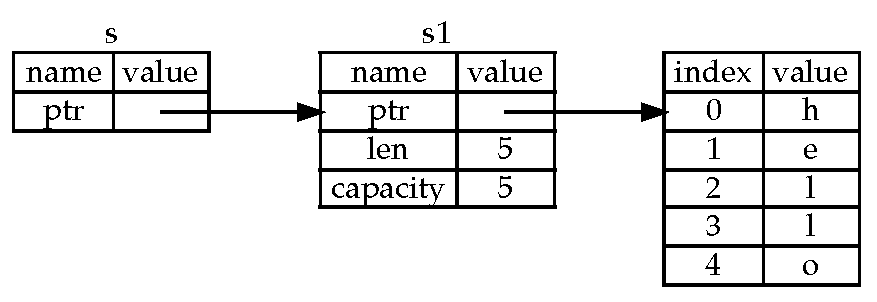
\includegraphics[scale=0.9]{Programmierung/Tabelle5.pdf}
    \caption{Diagramm von \texttt{\&String} \texttt{s} Zeiger auf \texttt{String} \texttt{s1}}
    \label{fig:tabelle5}
\end{figure}

Mit der \verb"&s1" Syntax kann eine Referenz erstellt werden, die sich auf den Wert von \verb"s1" bezieht, ihm aber nicht gehört. Der Wert den er verweist, wird nicht gelöscht, wenn die Referenz den Gültigkeitsbereich verlässt.

Ebenso verwendet die Signatur der Funktion \verb"&" um anzuzeigen, dass der Typ des Parameters eine Referenz ist.

Das Gegenteil der Referenzierung mit \verb"&" ist die Dereferenzierung, die mit dem Dereferenzierungsoperator \verb"*" erzielt wird.

Der Gültigkeitsbereich von \verb"s" ist der eines normalen Funktionsparameters. Jedoch wird der Wert nicht aus dem Speicher gelöscht, da keine Ownership an \verb"s" übergeben wurde, weshalb auch keine zurückgegeben werden muss. Referenzen als Funktionsparameter wird in Rust \glqq Borrowing\grqq{} genannt. Wie in der realen Welt kann Eigentum an andere ausgeliehen werden und wenn die andere Person es nicht mehr braucht, kann diese es wieder an den Eigentümer zurückgegeben.

Genauso wie Variablen standardmäßig unveränderlich sind, gilt dies auch für Referenzen. Es kann nichts verändert werden, auf das nur referenziert wird. Folgender Code würde also nicht funktionieren:

\begin{lstlisting}
    fn main() {
        let s = String::from("hello");
        change(&s);
    }
    fn change(some_string: &String) {
        some_string.push_str(", world"); // error
    }
\end{lstlisting}

\subsubsection{Veränderbare Referenzen}

Kleine Veränderungen beheben den Fehler aus dem letzten Programm:

\begin{lstlisting}
    fn main() {
        let mut s = String::from("hello");
        change(&mut s);
    }
    fn change(some_string: &mut String) {
        some_string.push_str(", world"); // works now
    }
\end{lstlisting}

Die Variable \verb"s" muss veränderbar sein mit \verb"mut". Es wird nun eine veränderbare Referenz übergeben und die Funktion erwartet auch einen entsprechende Referenz mit \verb"some_string: &mut String".

Veränderbare Referenzen haben eine große Einschränkung: Sie können nur eine veränderbare Referenz auf ein bestimmtes Datenelement in einem bestimmeten Bereich haben. Folgender Code würde also nicht funktionieren:

\begin{lstlisting}
    let mut s = String::from("hello");
    let r1 = &mut s;
    let r2 = &mut s;
    println!("{}, {}", r1, r2);
\end{lstlisting}

Diese Einschränkung erlaubt kontrollierte Veränderbarkeit von Variablen. Mithilfe dieser Regel verhindert Rust sogenannte \glqq data races\grqq{}. Diese ähneln sich einer \glqq race condition\grqq{} und tritt auf, wenn drei Verhaltensweisen auftreten:

\begin{itemize}
    \item Zwei oder mehr Pointer greifen zeitgleich auf den selben Speicherbereich zu.
    \item Mindestens einer der Pointer schreiben.
    \item Kein Mechanismus wird verwendet, um den Zugriff der Daten zu synchronisieren.
\end{itemize}

Diese \glqq data races\grqq{} können undefiniertes Verhalten auslösen und sind schwer festzustellen und zu beheben. In Rust-Programmen gibt es dieses Problem nicht, da gefährdeter Code nicht ohne Fehler kompiliert.

Es dürfen auch keine Kombinationen aus veränderbaren und unveränderbaren Referenzen erstellt werden. Folgender Code führt zu einem Compilerfehler:

\begin{lstlisting}
    let mut s = String::from("hello");
    let r1 = &s; // no problem
    let r2 = &s; // no problem
    let r3 = &mut s; // big problem
    println!("{}, {}, and {}", r1, r2, r3);
\end{lstlisting}

Bei unveränderliche Referenzen sollten man nicht damit rechnen müssen, dass sich der Wert dahinter verändern kann. Mehrere unveränderbare Referenzen sind in Ordnung, da mehrere lesende Zugriffe sich untereinander nicht beeinflussen.

\subsubsection{\glqq Dangling References\grqq{}}

In Programmiersprachen mit Pointer kann es vorkommen, dass Pointer auf einen Bereich im Speicher zeigen, der bereits freigegeben wurde, sogenannte \glqq dangling pointer\grqq{}. In Rust garantiert der Compiler, dass Referenzen immer auf einen gültigen Bereich zeigen. Folgender Code wird also beim Kompilieren eine Fehlermeldung ausgeben:

\begin{lstlisting}
    fn main() {
        let reference_to_nothing = dangle();
    }
    fn dangle() -> &String {
        let s = String::from("hello");
        &s
    }
\end{lstlisting}

Der String \verb"s" wird nach der Funktion \verb"dangle" aus dem Speicher gelöscht. Die Referenz, die zurückgegeben wird, würde auf einen ungültigen Bereich im Speicher zeigen. Der Compiler erkennt, dass der Rückgabewert eine \glqq dangling reference\grqq{} ist und gibt eine Fehlermeldung aus. Es sollte die Ownership von \verb"s" zurückgegeben werden, damit der String im Speicher bleibt:

\begin{lstlisting}
    fn no_dangle() -> String {
        let s = String::from("hello");
        s
    }
\end{lstlisting}

\subsubsection{Regeln: Referenzen}

\begin{itemize}
    \item Es kann entweder nur eine veränderbare oder eine beliebige Anzahl an unveränderlichen Referenzen benutzt werden.
    \item Referenzen müssen immer gültig sein.
\end{itemize}

\subsection{Slice Typ}

Ein weiterer Datentyp, welcher keine Ownership annimmt sind Slices. Sie wird benutzt um eine zusammenhängende Folge von Elementen einer Sammlung anstatt auf die gesamte Sammlung zu verweisen.

\subsubsection{String Slice}

Wenn ein bestimmter Teil eines String referenziert werden soll, würde man in andern Sprachen den Index berechnen, an welcher Stelle z.B. ein neues Wort beginnt. Wenn der String jedoch vom Speicher gelöscht wird, existiert der berechnete Index immer noch, da er nach der Berechnung unabhängig geworden ist.

In Rust kann mit sogenannten \glqq string slices\grqq{} ein bestimmter Bereich eines Strings referenziert werden.

\begin{lstlisting}
    let s = String::from("hello world");
    let hello = &s[0..5];
    let world = &s[6..11];
\end{lstlisting}

Die Syntax der Klammern beschreibt \verb"[starting_index..ending_index]". Intern wird die Startposition und Länge gespeichert. Die Länge ergibt sicht aus der Differenz aus \verb"starting_index" und \verb"ending_index". Die Variable \verb"world" ist ein Pointer auf das siebte Byte von \verb"s" mit einer Länge von 5. \autoref{fig:tabelle6} zeigt ein Diagramm des Speichers.

\begin{figure}[htbp]
    \centering
    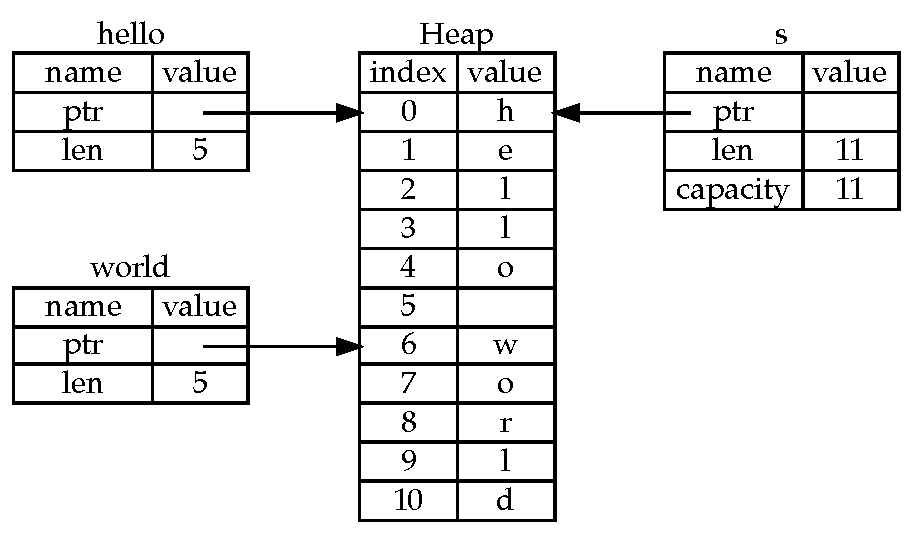
\includegraphics[scale=0.9]{Programmierung/Tabelle6.pdf}
    \caption{Diagramm eines String Slice}
    \label{fig:tabelle6}
\end{figure}

Dadurch entsteht eine Abhängigkeit, welche es Rust erlaubt, bereits beim Kompilieren festzustellen, ob String Slices auf einen gültigen Bereich zeigen. So wird der Code weniger anfällig für Laufzeitfehler.

\begin{lstlisting}
    let s = "Hello, world!";
\end{lstlisting}

Der Typ von \verb"s" ist \verb"&str": Es ist ein String Slice, welcher auf einen bestimmten Punkt zeigt. Deshalb sind String-Literale unveränderlich. \verb"&str" ist eine unveränderliche Referenz.

\subsubsection{Andere Slices}

String Slices sind spezifisch für Strings. Es gibt auch einen allgemeineren Slice-Typ. Genauso wie bei Strings, können auch Teile von Arrays referenziert werden:

\begin{lstlisting}
    let a = [1, 2, 3, 4, 5];
    let slice = &a[1..3];
\end{lstlisting}

Der Typ von \verb"slice" ist \verb"&[i32]". Auch hier wird ein Pointer auf das erste Element gespeichert sowie die Länge des Slice.


% BibTex mit Stil alpha
\nocite{*}
\bibliography{Bibliothek}{}
\bibliographystyle{alpha}

% Abbildungsverzeichnis, Tabellenverzeichnis und Glossar ausgeben
\listoffigures
\listoftables
\printglossaries 

\end{document}
